\section{Анализ полученных результатов теплового режима РЭС}
\subsection{Обработка и анализ данных проведенного результата}

Гораздо легче принимать конструкторские решения обладая визуальным
представлением данных. По это причине данный раздел в основном состоит
из гистогорамм отображающих в результаты расчетов температур.




\subsubsection{Анализ тепловых режимов для корпуса блока:}
\begin{figure}[h] %% h means here
\begin{center}
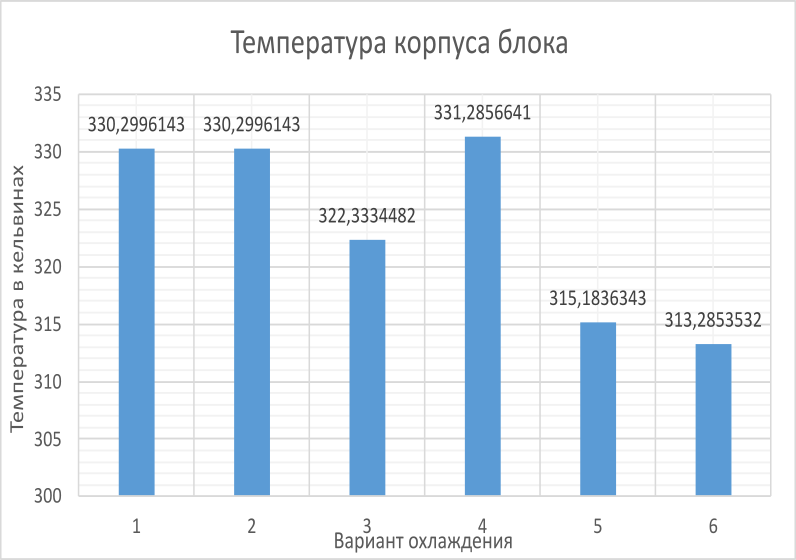
\includegraphics[scale = 0.4]{t_corp.png}
\caption{Температура корпуса блока:\\
  1 - тепловой режим герметичного корпуса\\
  2 – тепловой режим блока в герметичном корпусе с внутренним перемешиванием\\
  3 – тепловой режим блока в герметичном корпусе с наружным обдувом\\
  4 - телповой режим блока в  герметичном оребренном корпусе \\
  5 – тепловой режим блока в перфорированном корпусе \\
  6 - тепловой режим блока при принудительном охлаждении}
\end{center}

\end{figure}

На гистогорамме ожидаемо оказались равными значения температур для
герметичного корпуса и для корпуса с внутренним перемешиванием. Это
обусловлено тем, что скорость перемешивания при расчете была равна
нулю и закономерно.

Неожиданно то, что значения температур при принудительном и охлаждении
и при использовании оребренного корпуса оказались выше, нежели те же
значения для режима с обдувом и использовании перфорированного корпуса.

С другой стороны, можно обосновать низкую температуру корпуса при
обдуве тем, что при таком методе охлаждения набегающим потоком воздуха
тепло отводится в первую очередь от корпуса.

Самым эффективным оказалось использование перфорированного корпуса.
Это настораживает, так как принудительное охлаждение считается по
определению самым эффективным и поэтмум возникают вопросы
к правильности рассчета, когда самая низкая температура оказывается в
тепловом режиме с перфорированием.\\


\subsubsection{Анализ тепловых режимов для поверхности элемента:}
\begin{figure}[h] %% h means here
\begin{center}
  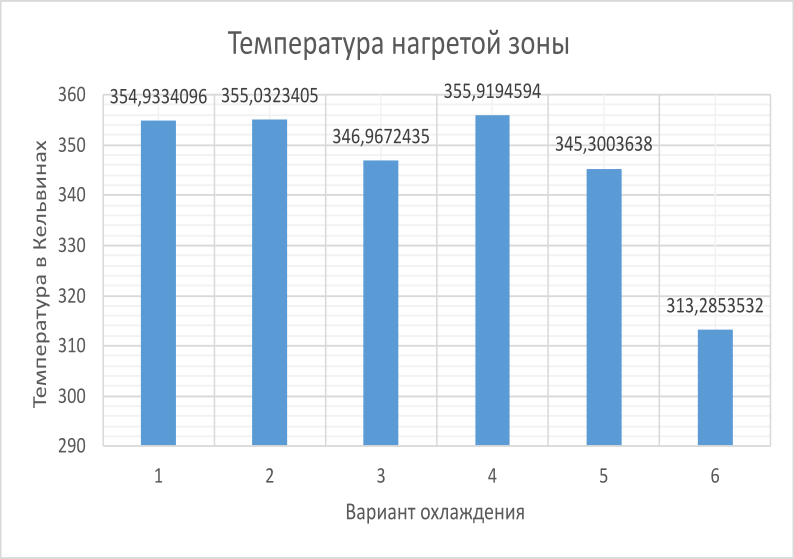
\includegraphics[scale = 0.4]{t_surface.png}
  \end{center}
\caption{Температура поверхности элемента:\\
  1 - тепловой режим герметичного корпуса\\
  2 – тепловой режим блока в герметичном корпусе с внутренним перемешиванием\\
  3 – тепловой режим блока в герметичном корпусе с наружным обдувом\\
  4 - телповой режим блока в  герметичном оребренном корпусе \\
  5 – тепловой режим блока в перфорированном корпусе \\
  6 - тепловой режим блока при принудительном охлаждении}

\end{figure}

Ожидаемое самым низким оказалась температура в телповом режими с
принудительным охлажденим.

Однако температура при расчете для
теплового режима блока в оребренном корпусе оказалось выше, даже чем
тепловой режим герметичного корпуса, что объяснить сложно. Это также
может свидетелсьтвовать об ошибках вычислениях.

\subsubsection{Анализ тепловых режимов для воздуха в блоке.}
\begin{figure}[h] %% h means here
\begin{center}
  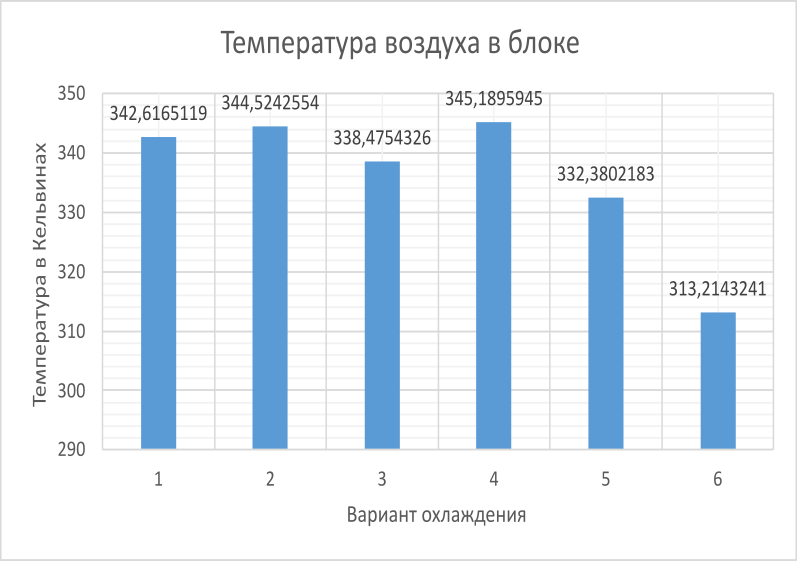
\includegraphics[scale = 0.4]{t_air.png}
  \end{center}
\caption{Температура воздуха блоке:\\
  1 - тепловой режим герметичного корпуса\\
  2 – тепловой режим блока в герметичном корпусе с внутренним перемешиванием\\
  3 – тепловой режим блока в герметичном корпусе с наружным обдувом\\
  4 - телповой режим блока в  герметичном оребренном корпусе \\
  5 – тепловой режим блока в перфорированном корпусе \\
  6 - тепловой режим блока при принудительном охлаждении}

\end{figure}

На данной графике самым эффективным оказывается режим с принудительным
воздушным охлажденим, что закономерно.

Однако, на графике видно, что при перемешивании температура воздуха выше,
чем при его отсуствие.

В прочем, сложно сказать достоверно ли это, так как при расчете
скорость перемешивания взята равной нулю, что обусловлено тем, что
охлаждение естественное.


На этом этапе становится анализа становятся очевидн
\begin{enumerate}[label={\arabic*.}]

\item Самое эффективный способ охлаждения из рассмотренных
  — принудительное воздушное охлаждение.
\item Значения первых двух тепловых режимов, то есть теплового режима
  герметичного корпуса и герметичного корпуса с перемешиванием в
  большинстве случаев будут выше чем значения в остальных температурных режимах.
  
\end{enumerate}

    Это означает, что более пристальному анализу подлежат только
    третий, четвёртый и пятый режимы,
    соответвенно обеспечивающие охлаждение

\subsubsection{ Анализ тепловых режимов окружающей элемент среды.}
\begin{figure}[h] %% h means here
\begin{center}
  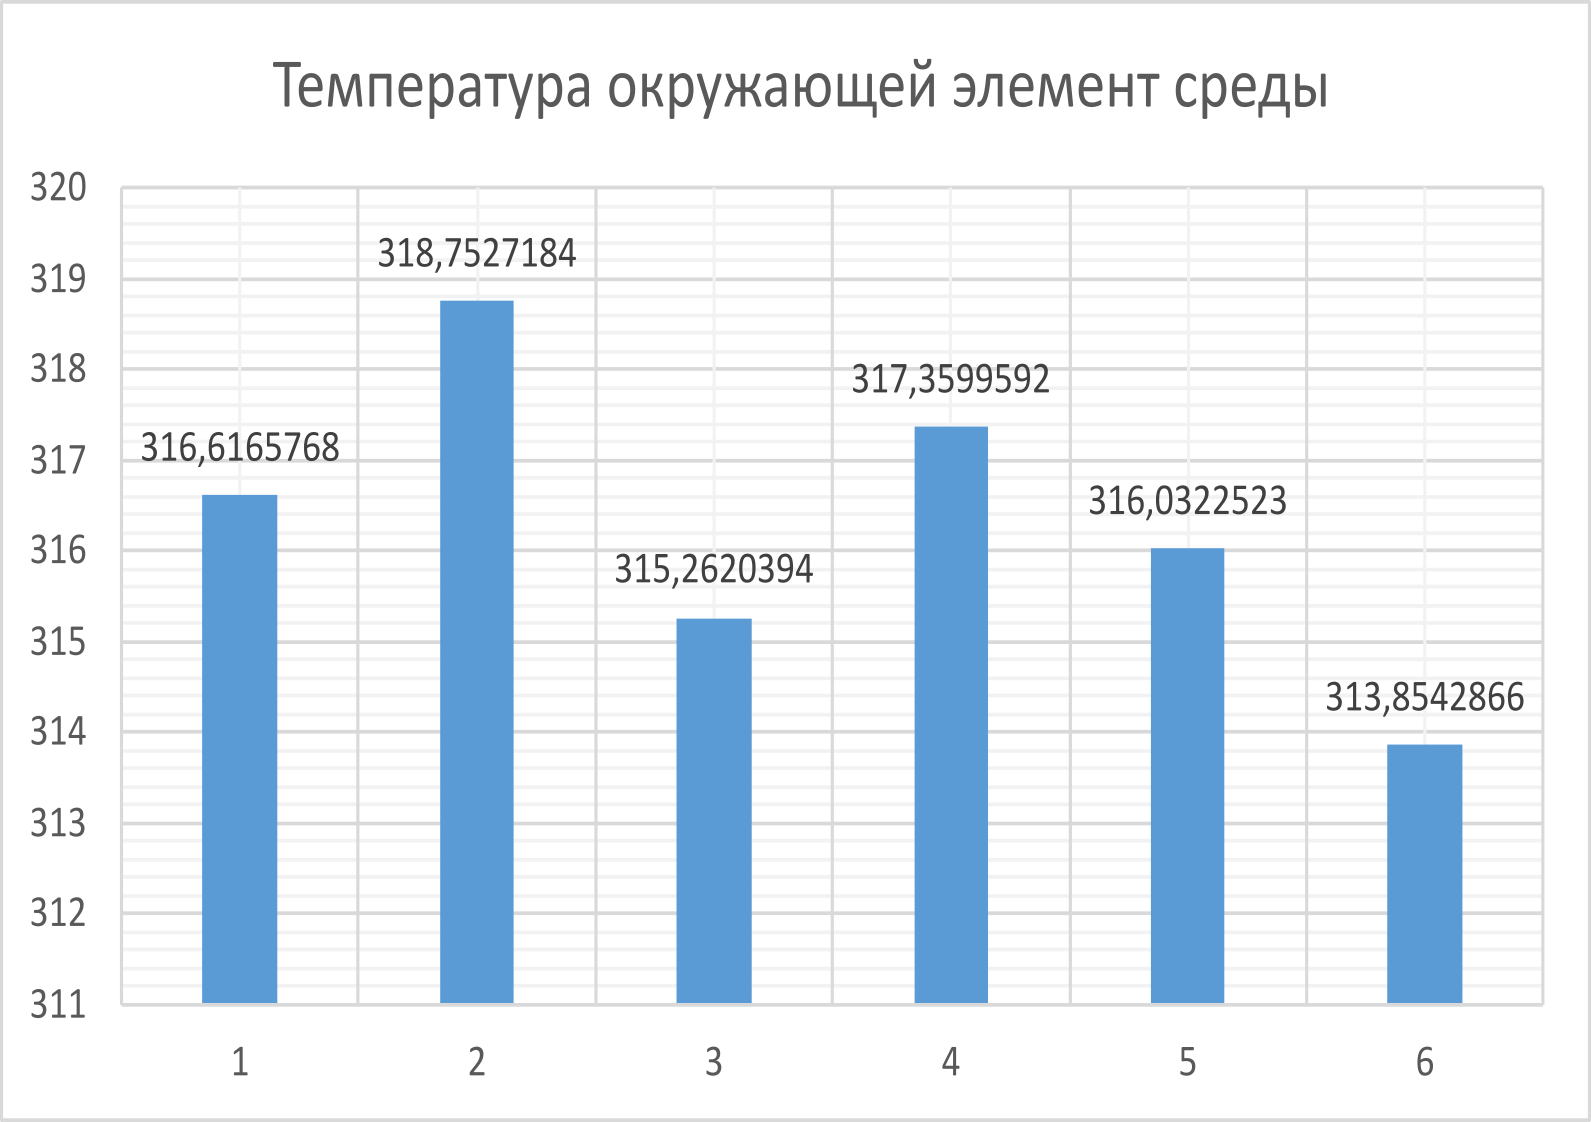
\includegraphics[scale = 0.4]{t_env.png}
  \end{center}
\caption{Температура окружающей элемент среды:\\
  1 - тепловой режим герметичного корпуса\\
  2 – тепловой режим блока в герметичном корпусе с внутренним перемешиванием\\
  3 – тепловой режим блока в герметичном корпусе с наружным обдувом\\
  4 - телповой режим блока в  герметичном оребренном корпусе \\
  5 – тепловой режим блока в перфорированном корпусе \\
  6 - тепловой режим блока при принудительном охлаждении}

\end{figure}

Данная гистограмма выглядит,
как наиболее близкая к действительным значениям,
если не учитывать разницу между тепловым режимом герметичного корпуса
и корпуса с перемешиваеним, при котором, в корпусе с перемешиваеним
оказывается большая температура.

\subsubsection{Анализ тепловых режимов  для
воздуха в блоке при способах охлаждения с помощью наружного обдува,
оребренным корпуса и перфорацией.}

\begin{figure}[h] %% h means here
\begin{center}
  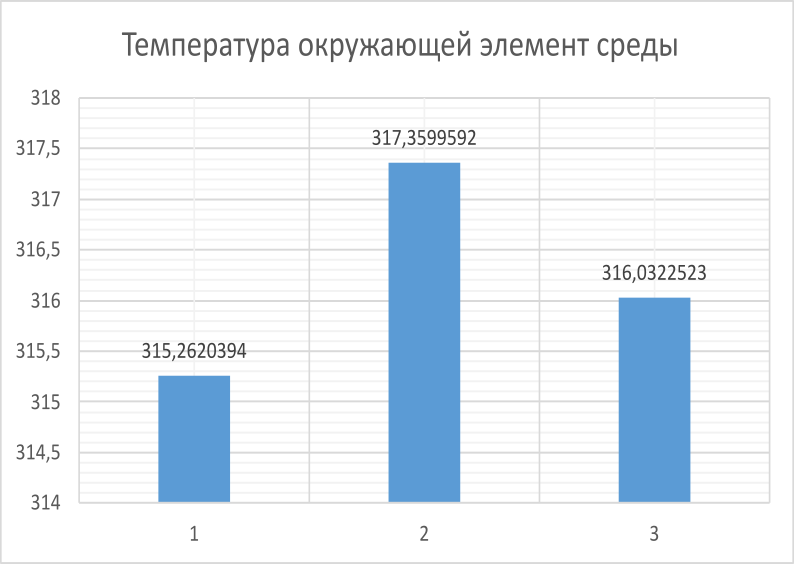
\includegraphics[scale = 0.4]{t_env_2.png}
  \end{center}
\caption{Температура воздуха в блоке:\\
  1 – тепловой режим блока в герметичном корпусе с наружным обдувом\\
  2 - телповой режим блока в  герметичном оребренном корпусе \\
  3 – тепловой режим блока в перфорированном корпусе \\
}

\end{figure}

На данной гистограмме видно, что наиболее эффективным из оставшихся
является охлаждение с наружным обдувом.

\subsubsection{Анализ тепловых режимов для окружающей элемент среды при
способах охлаждения с помощью наружного обдува, оребренным корпусом и
перфорацией.}

\begin{figure}[h] %% h means here
\begin{center}
  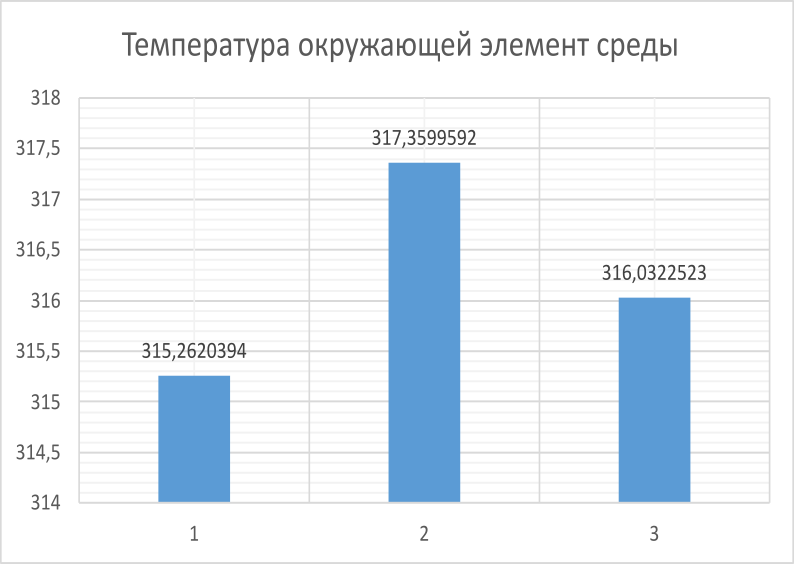
\includegraphics[scale = 0.4]{t_env_2.png}
\end{center}
\caption{Температура окружающей элемент среды:\\
  1 – тепловой режим блока в герметичном корпусе с наружным обдувом\\
  2 - телповой режим блока в  герметичном оребренном корпусе \\
  3 – тепловой режим блока в перфорированном корпусе \\
}

\end{figure}

Данная гистограмма также показывает охлажденим наружным обдувом как
самое эффективное.

На основании этого можно сделать заключение, что самым эфективным
после принудительного воздушного является метод охлаждения обдувом.
Конструкторами же устройства выбран метод охлаждения за счет
перфорации корпуса, который, является вторым по эффективности рассеивания тепла
и может быть предпочтительным.

\subsubsection{Моделирование теплового режима в elcut}

Было проведено моделирование печатной теплового режима печатной платы
в elcut.


\begin{figure}[h]
  \centering
  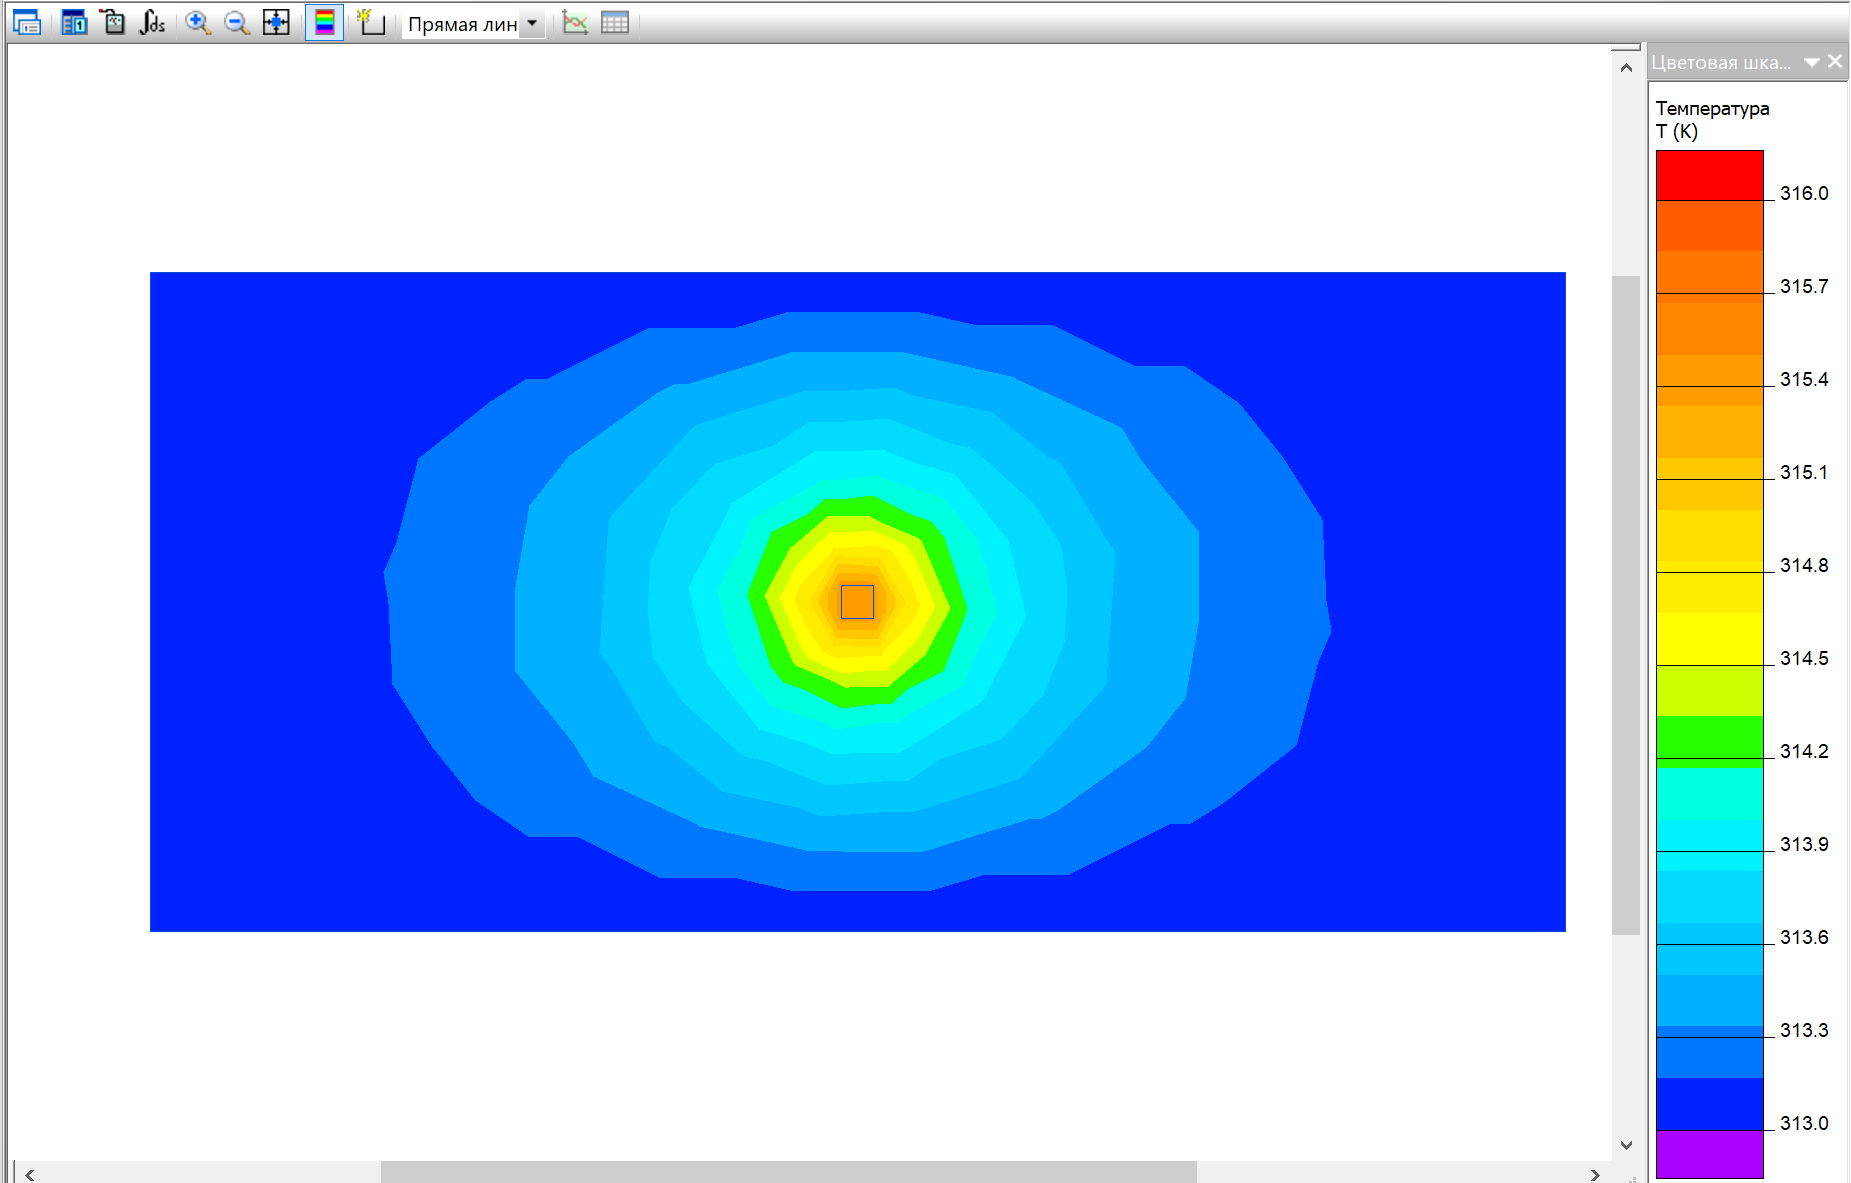
\includegraphics[scale = 0.30]{elcut_solved}
  \caption{
    Результат решения задачи теплопроводности в elcut. }
\end{figure}

В результате решения задачи тепловроднотси в elcut можно сделать
вывод, что за счет большой площади печатной платы происходит
рассеивание большей части тепловой энергии.

Это свидетельствует о том, что в данном конретном случае выбор
конкретного способа охлаждения не принципиален и использование не
самого эффективного его варианта, а именно использование корпуса с
охлажденим достаточно для решения задачи по обеспечению теплового
режима. 